\section{Method}

\subsection{Source of data}

For this comparative study the following data sources will be used

\begin{enumerate*}
	\item \gls{ac:nibio}
	\item Xgeo
	\item \gls{ac:kilden}
	\item \gls{ac:met}
\end{enumerate*}

\subsection{Dataset}

The dataset is chosen from four regions in Norway; Innlandet, Vestfold, Trøndelag, and Østfold. From each region are four stations picked:
\begin{table}[h]
	\begin{adjustwidth}{-1in}{-1in}
		\centering
		\begin{tabular}{ccccccccc}
			\hline Region&Name&ID&Drain type&Soile category&Texture&MET name& Latitude&Longdetude\\\hline
			Innlandet&Apelsvoll&11& Selvdrenert&CM& 17&SN11500&60,70024&10,86952\\
			Innlandet& Fåvang&17& Selvdrenert&CM& 15&SN13150&61,45822&10,1872\\
			Innlandet& Ilseng&26& Selvdrenert&PH& 17&SN12180&60,80264&11,20298\\
			Innlandet& Kise&27& Vannmettet&GL& 99&SN12550&60,77324&10,80569\\
			Trøndelag& Kvithamar&57& Vannmettet&ST& 16&SN69150&63,48795&10,87994\\
			Trøndelag& Frosta&15& Selvdrenert&LP& 13&SN69655&63,56502&10,69298\\
			Trøndelag& Mære&34& Selvdrenert&RG& 14&SN71320&63,94244&11,42527\\
			Trøndelag& Rissa&39& Vannmettet&PL& 13&SN71320&63,58569&9,97007\\
			Vestfold& Lier&30& Vannmettet&ST& 16&SN19940&59,79084&10,25962\\
			Vestfold& Sande&42& Vannmettet&ST& 16&SN26990&59,6162&10,22339\\
			Vestfold& Tjølling&50& Selvdrenert&AR& 13&SN27780&59,04641&10,12513\\
			Vestfold& Ramnes&38& Vannmettet&ST& 16&SN27315&59,38081&10,2397\\
			Østfold& Rakkestad&37& Vannmettet&ST& 18&SN3290&59,38824&11,39042\\
			Østfold& Rygge&41& Selvdrenert&AR& 13&SN17380&59,39805&10,75427\\
			Østfold& Tomb&52& Vannmettet&ST& 16&SN17050&59,31893&10,81449\\
			Østfold& Øsaker&118& Vannmettet&ST& 18&SN3370&59,31936&11,04221\\\hline
		\end{tabular}
	\end{adjustwidth}
	\caption[Soil information for each station/w location and MET-ID]{Station information from stations used in this study. The texture class is defined in this article: https://nibio.no/tema/jord/jordkartlegging/jordsmonnkart/dominerende-tekstur-i-overflatesjikt}
\end{table}

All stations are sampled from the date\footnote{Format month-day} 03-01 to 10-31 from 2016 to 2020. The features rain (RR), mean soil temperature at 10cm (TJM10), mean soil temperature at 20cm (TJM20), and air temperature at 2m (TM) are sampled from the LMT database. The snow parameter is sampled from MET via Xgeo for imputed values in areas where there are no messured values. The soil type, and soil texture is sampled from Kilden from Norwegian Institute of Bioeconomy Research.

\subsubsection{Selection process}
The selection process for finding these station can be compiled into these steps

\begin{enumerate}
	\item Recommendation from Norwegian Institute of Bioeconomy Research
	\item \label{list:na_anal}Compute the missing values in the data
	\item Missing values analyse 
	\item Searching LMT database for alternative station candidates if current data is insufficient
	\item If some station was replaced the repeat step \ref{list:na_anal}
\end{enumerate}

\begin{figure}
	\centering
	\label{fig:plot-17}
	\includegraphics[width=0.8\linewidth]{"../../results/plots/Plot_test_naive_nan_k17_fTJM20.pdf"}
	\caption[Visual representation of station 17]{Visual representation of missing values at station 17 from 2014 to 2022 at the parameter "TJM20". The left numbers indicated how many hours that are missing and how many of them are shorter than or longer than 5 hours. The yellow markings indicate possible outliers based on the given year, all markings was checked if they were actual outliers. The red colouring indicate missing values in the data (represented in the data with code "NULL").}
\end{figure}

The plots of stations follow a simple representation where the y-axis represent the year and the x-axis represent the index of the data as all tables are taken from the same period. A circle represent a singluar na values, while a band represent a series of 2 or more missing values. The colours represents the features used in this comperative study. This representation of the missing values will indicate sesonal, and systematic removal of data and give an overall indication of how much data is missing. To get further insight into the data a report is generated in parallel to the plots describing precise date and time of all values and which other parameter values is also missing values in the same period. See appendix \ref{apx:code:dataanal} for the full detail of the report generation and appendix \ref{apx:plots} for na-plots of the station chosen for this study.

\subsubsection{Collection of data}

The method used was a powershell\footnote{Version 7.3.11} script that called the respective institutions servers using the "curl" program\footnote{curl 8.4.0 (Windows) libcurl/8.4.0 Schannel WinIDN} to send an http request for the timeseries starting from 2014 to 2020 in the interval 1 of May to 31 of October. Code for data collection can be viewed in appendix \ref{apx:code:datacollect}. The data is stores as an either a csv file or a json file for easy retrieval and manual control of values.

\subsubsection{Labeling of stations between Nibio and MET}
\begin{table}
	\centering
	\begin{tabular}{r|p{5cm}|}
		FROST & Description\\\hline
		Stations with rain & Requested rain data in millimeters. \\
		Station ID & Sendt a request to LMT for station information using their remote API. \\
		\hline LMT & Description \\\hline
		Meteorological data & Requested soil temperature from 10cm depth, and 20cm depth and air temperature (2m), from 2014-03-01 to 2022-10-31.\\
	\end{tabular}
	\caption[Request to servers about stations]{Description of what was requested from each server (FROST part of \acrshort{ac:met}, \acrshort{ac:nibio}).}
	\label{tab:station_request}
\end{table}

Since Nibio and MET have different names for the same stations one must compile a list that converts Nibio ID to MET ID. This was performed with these requests shown in table \ref{tab:station_request} where ID is the Nibio Id for the given station, Frost.ID is the MET id, ID. latitude is the latitude gathered from Nibio, ID.longitude is the longitude gathered from Nibio. These variables can be swaped out for the relevant station.\todo{Move to caption}

\subsubsection{Storage of data}
The storage of the data is done through two data structures; \gls{gl:hashmap} and \gls{gl:dataframe} from the package pandas. The transformation of data is done with a costume datatype called "DataFileHandler" which is converted to a module for convenience. The keys for the hashmap is chosen by the naming of the data files and the pattern given to the class. To escalete modeling the data will also be exported to a binary file for faster retrieval. \todo{MORE DETAIL}

\begin{figure}
	\centering
	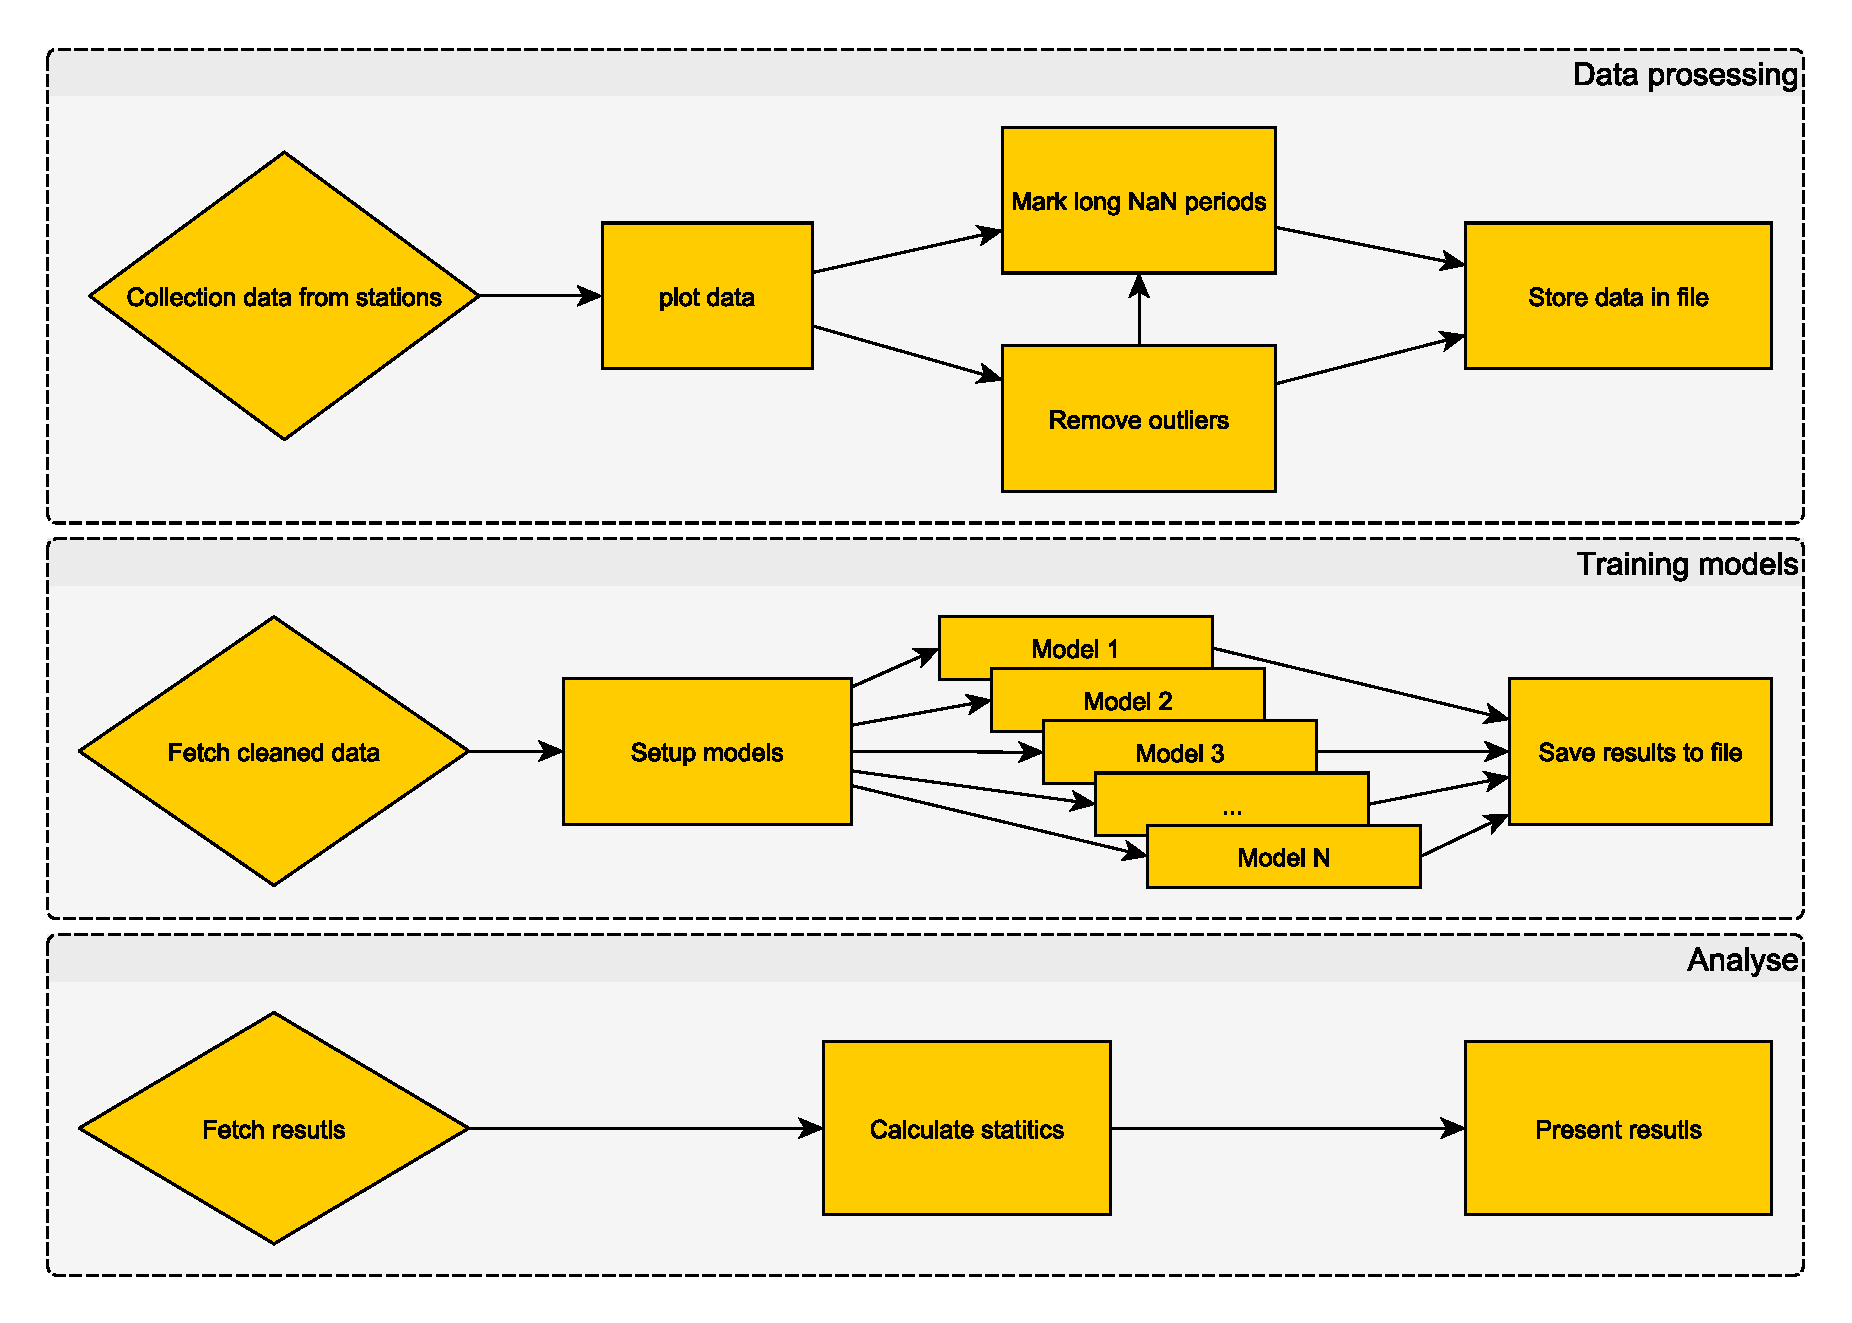
\includegraphics[width=0.7\linewidth]{figures/progress_diagram}
	\caption[Diagram sketching three procedures used in this study.]{A surface level diagram of the }
	\label{fig:progressdiagram}
\end{figure}\todo{Complete diagram}


\paragraph[Data structure]{Technical overview of custom data structure}
The data structure used to store the data from the different stations is called "DataFileHandler" and stores the data in a tree-structure where indexes are dictated by the filename. It has several built-in functions to assist with data partitioning, and merging of data. This makes it easier to move and store all 846 720 observations from 16 station from all 4 regions\footnote{there are 4 stations per region.}. Further more, the data structure has iteration functions so it is compatible with python's built in loops, and print functions. 

\subsection{Data cleaning and treatment}

To use the data in this study it must be cleaned and treated for training. The following methods were picked common practice in litterateur with new methods based on the decomposition of the data in the from of \acrfull{ac:stl}\cite{cleveland_stl_1990}\footnote{In this study we expand this for multiple seasons using \acrfull{ac:mstl}\cite{bandara_mstl_2021}, but the theory of this imputation method remains the same.}.

\subsubsection{Outlier detection and removal}\todo{Revise so it reflects what you actialy do}

Though the data fetched from \acrshort{ac:nibio} is treated and controlled the external data from \acrshort{ac:met} might not be, and this research project incorporated raw, untreated data from \acrshort{ac:nibio} to fill inn missing values.

The method to quickly find obvious outliers was to look at the following condition
$$
	|\frac{|\Delta T|-µ(|\Delta T|)}{var(|\Delta T|)}|> 4℃
$$\todo{Make more clear}

This condition looks at the absolute difference between consecutive measurements and calculates the z-score for each observation. It is expected that the change in temperature can't be too rapid. Further methods used to highlight potential outliers is 

\begin{figure}[h]
	\centering
	\definecolor{zzttqq}{rgb}{0.6,0.2,0.}
	\definecolor{REDDD}{rgb}{0.8,0.5,0.2}
	\definecolor{ududff}{rgb}{0.30196078431372547,0.30196078431372547,1.}
	\begin{tikzpicture}[line cap=round,line join=round,>=triangle 45,x=1.0cm,y=1.0cm]
		\begin{axis}[
			x=1.0cm,y=1.0cm,
			axis lines=middle,
			ymajorgrids=true,
			xmajorgrids=true,
			xmin=-0.5,
			xmax=3.5,
			ymin=-0.5,
			ymax=2.5,
			xtick={-0.0,1.0,...,3.0},
			ytick={-0.0,1.0,...,2.0},]
			\clip(-0.5,-0.5) rectangle (3.5,2.5);
			\draw [line width=2.pt,dash pattern=on 1pt off 1pt] (1.04,1.02)-- (3.04,0.02);
			\draw [line width=2.pt] (1.04,1.02)-- (2.04,2.02);
			\draw [line width=2.pt] (2.04,2.02)-- (3.04,0.02);
			\begin{scriptsize}
				\draw [fill=ududff] (1.04,1.02) circle (2.5pt);
				\draw[color=ududff] (1.18,1.39) node {$A$};
				\draw [fill=ududff] (3.04,0.02) circle (1.5pt);
				\draw[color=ududff] (3.18,0.31) node {$B$};
				\draw [fill=ududff] (2.04,2.02) circle (1.5pt);
				\draw[color=ududff] (2.18,2.31) node {$C$};
				\draw [fill=zzttqq] (2.,0.54) circle (2.5pt);
				\draw [color=REDDD,dashed] (2.,0.54) circle (0.5);
				\draw[color=zzttqq] (2.14,0.91) node {$C^*$};
			\end{scriptsize}
		\end{axis}
	\end{tikzpicture}
	\caption[Simple Interpolation outlier detection]{An simple outlier detection method utilizing a simple line to estimate where the expected point ($C^*$) is supposed to be. If observed point C falls outside the tolerance level (red dotted circle) then it is marked as an outlier.}
\end{figure}

\subsubsection{Missing value imputation}

The data has missing values, in particular during early Fall when there were sub-zero temperatures meaning any rain measurements done during this period would have unpredictable fluctuations since at negative temperatures water can freeze, get clogged up with residual bio-material from the surrounding area \todo{Rewrite this part to reflect what is going on}

\subsection{Setup of models}\todo{In general, write more on all subsections}

The models are set up in according to the relevant paper the model is fetched from, alternatively reuse the code made by the author. When importing the data to the model there will be modifying to the original code to facilitate for the model as far as it goes. Any modifications will be in the appendix under section \ref{apx:code}. For the convenience of the reader all code is using the sklearn estimator class to make all the models discuses in this study more user friendly and compatible with sklearns other functions. The details of the models will be discussed in section \ref{sec:theory}, this section discusses the setup and implementation of the models.\footnote{Caution to the reader; The code used was run on the Linux subsystem (Debian) on windows due to the fact that the current version of tensorflow can't run on Windows.}

\subsubsection{Basic Linear model}

The linear model (sec \ref{sec:theory:linreg}) utilises in the study is created from the python model sklearn (or scikit-learn according to pythons package manager) 

\subsubsection{Plauborg}

The Plauborg regression will be formulated as a linear regression problem so that the LinearRegression function in the Sci-kit module can be used. For the parameters used in the paper\cite{plauborg_simple_2002} the F function defined in section \ref{sec:theory:pluborg} will be formulated with loops to give rise 3 more parameters for fine-tuning the model.

\subsubsection{BiLSTM}

\begin{figure}
	\centering
	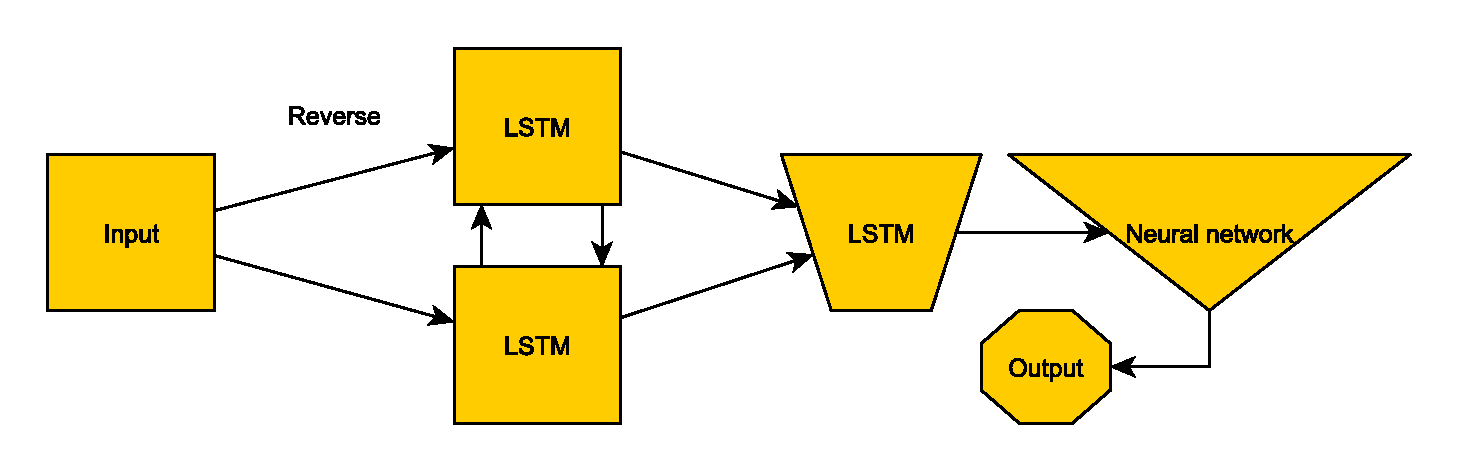
\includegraphics[width=0.7\linewidth]{figures/BiLSTM}
	\caption[BiLSTM overview]{}
	\label{fig:bilstm}
\end{figure}\todo{Complete caption, and improve figure}

Soil temperatures are dependent on earlier timestemps meaning that to make a good prediction one needs to include temperature from $t,t-1,\dots,t-k$ to make a decent prediction. As a base model it is usefull to evalueate the data both forwards and backwards to find features that is only notisable in a sertan direction. The BiLSTM defined is crafted with Tensorflow's Keras module for ease of use. 

\subsubsection{Attention-aware ILSTM}

It is a know fact, since 1849\footnote{First weather prediction made by Joseph Henry in 1849}, that to know previous weather patterns will greatly improve prediction accuracy. To improve the accurasy even more a model can focus one specific patterns that has a big impact on the prediction. The ILSTM attempts to do this by including a new thecnick in data science called attention\cite{vaswani_attention_2017} that takes a collection of data and gives each element a weight associated with importance. When that paper was published it was focused on translation between English and German, however the paper published by \citeauthor{li_attention-aware_2022} uses this novel teknick to do both time and feature importance and from that make a prediction.

\subsection{Metrics}

The metrics used in this study are

\begin{itemize*}
	\item Mean Squere Error
	\item Mean Absolute Error
	\item Explained Variance
	\item bias
	\item Log Condition number
	\item digit sensitivity
\end{itemize*}


Soil temperatur as a differnet behavor than air temperature since energy (temperature) though the soil gets dampen and delayed. Since the data used in this study has outliers that was not cought during datatreatment, which has been addresed, the author of this study desided to include two more metrics that are not usually included in the evaluation; The log condition number, and digit sensitivity. Both metrics are based on the calculation of the condition number defined as 

\begin{equation}\label{eq:kappa}
\kappa = \lim\limits_{\varepsilon \to 0^+} \sup\limits_{|\partial x|\leq\varepsilon}  \frac{\left|f(x+\partial x) - f(x)\right|}{|f(x)|}*\frac{|x|}{|\partial x|} 
\end{equation}

This is not feasible to calculate since infinite calculations with infinitesimal numbers is not possible as per \today for simulation approach\footnote{This calculation is possible for some models, for instance linear regression models when converted to the form $A\vec{\beta} = \vec{y}$.}. Therefore this paper uses algorithm \ref{alg:cond_num} to approximate $\kappa$ for all the models.

\begin{algorithm}[H]
	\SetAlgoLined
	\KwData{ Data }
	\KwResult{log($\kappa$)}
	Let $\kappa_f$ be the function \ref{eq:kappa}\;
	$\kappa\gets 0$\;
	\For{$i \in {1 \dots |Data|}$}{
		$\partial x \gets \mathcal{U}_{[-\sqrt{\varepsilon/|Data|},\sqrt{\varepsilon/|Data|]}}$\;
		$k \gets$ calculate with $\kappa_f$ from $x$ and $x+\partial x$\;
		\If{k > $\kappa$}{$\kappa \gets k$\;}
	}
	\Return{$\kappa$}
	\caption[Randommised $\kappa$ algorithm]{Method for calculating $\kappa$. $\mathcal{U}$ is a uniform random distrebution in a range.}
	\label{alg:cond_num}
\end{algorithm}

The digit sensitivity is included to give an intitive understanding of $\kappa$ and is computed simply as $\log_e(\kappa)+1$. This number tells us the significant digit generated from the model. If the number is less than 0 then its the ith digit after the decimal point.

For the rest of the metrics, they are defined as follows
\begin{itemize}
	\item RMSE = $\sqrt{\frac{\sum (y_{\text{pred}} - y_{\text{truth}})^2}{n}}$
	\item MAE = $\frac{\sum \left| y_{\text{pred}} - y_{\text{truth}}\right|}{n}$
	\item bias = $\frac{\sum ( y_{\text{pred}} - y_{\text{truth}})}{n}$
	\item Explained variance = $1-\frac{\sum (y_{\text{pred}} - y_{\text{truth}})^2}{\sum (y_{\text{pred}} - \vec{y})^2}$
\end{itemize}

Where $\vec{y}$ is the mean of the target, $y_{\text{pred}}$ is the predicted data, and $y_{\text{truth}}$ is the observed soil temperature.

\subsection[Use of AI]{Use of Artificial Intelligence in this paper}

In this paper there has been used Artificial Intelligence (AI), specifically Bing Chat / Copilot hosted by Microsoft Cooperation with special agreement with \acrfull{ac:nmbu}, for the following purposes:

\begin{enumerate}
	\item Formalising sentences and rephrasing sentences.
	\item Spellchecking
	\item Code generation of basic consepts and structures (tree traversal, template for generic classes) 
\end{enumerate}

It is important to emphasize that our engagement with AI have been actively curated and verified with known information. All code underwent rigorous manual inspection within a dedicated testing environment. Furthermore, no confidential or sensitive information was shared with the AI; our interactions focused solely on broad topics and general inquiries. To validate the accuracy of AI-generated responses, we cross-referenced them with established research papers and textbooks.